\documentclass{article}

\title{Simulating and Reconstructing X-Ray CT Projections}
\author{Reece Garthwaite}
\date{}

\usepackage{graphicx}
\usepackage{amsmath}
\usepackage{pythonhighlight}
\usepackage{float}
\usepackage{url}

\begin{document}
\maketitle

\begin{abstract}
I have chosen to simulate x-ray transmission through a digital phantom, using energy dependent attenuation to generate sinograms that I then reconstruct using simple back projection. I used NIST data to model bone and soft tissue with energy dependent attenuation coefficients.
\end{abstract}

\section{Introduction}
Computed tomography scans are a form of medical imagery that uses X-rays to  create images of the body. CT scans reconstruct cross sectional images of the body from multiple projections of X-ray attenuation through an object. In this project, I go through a large amount of the process of X-ray imaging: from simulating the incident X-rays using the python software toolkit spekpy, to simulating the x-ray attenuation and forming a spectogram, I then reconstruct the image using simple back projection.

\section{Methods}

\subsection{Background Physics}
\subsubsection{X-ray generation}
X-rays are produced when high kinetic energy electrons are accelerated towards a positive anode in a x-ray tube. Tungsten is a common choice for the anode (due to its high melting point and high atomic number). Electrons come close to nuclei of the target, causing a deceleration and change in direction, converting kinetic energy into a spectrum of electromagnetic radiation. Incident electrons can ionise the material, removing an electron from the anode. As the electron orbit vacancy gets filled by a orbital shell electron in a further out shell a photon is emitted. As orbital energies and their differences are unique in atoms, this leads to what we call "characteristic radiation".
\cite{Tafti}

\begin{figure}
  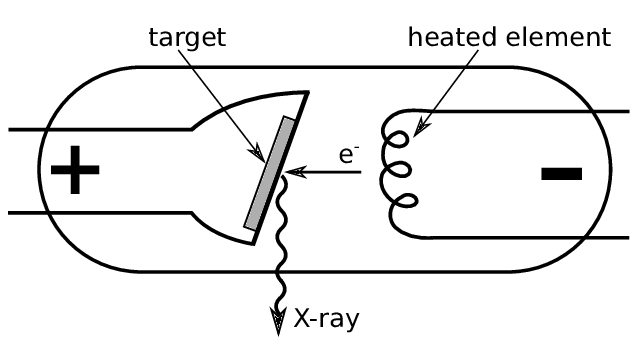
\includegraphics[width=\linewidth]{xray_tube.png}
  \caption{A X-ray tube}
  \label{fig:X-ray tube}
\end{figure}
Figure \ref{fig:X-ray tube} \cite{Mason} shows a diagram of a X-ray tube . Which helps to visualise the origin of the X-ray spectrum as electrons are emitted via thermionic emission and then accelerated toward a positively charged anode, where their interactions with the target produce both bremsstrahlung and characteristic radiation.

\subsubsection{Attenuation of X-rays}
As X-rays pass through matter, they are attenuated according to the Beer-Lambert law: 
\begin{equation} \label{bl}
I(E) = I_0 \cdot e^{-\mu(E) x}
\end{equation}

Where:
\begin{itemize}
  \item I = transmitted intensity of radiation after passing through the material
  \item $I_0$ : Initial intensity
  \item $\mu$ : Linear attenuation coefficient
  \item $x$ : Thickness of material
\end{itemize}

I have included  $\mu$ to be energy dependent as this is what is observed in experiments, and allows us to look for an interesting phenomenon known as beam hardening. I calculate $\mu$ using:
\begin{equation} \label{linearatt}
\mu(E) = \left(\frac{\mu}{\rho}\right) \cdot \rho
\end{equation}
using mass attenuation data from NIST and known material densities.

\subsection{Investigating Beam Hardening}
Beam hardening occurs during X-ray attenuation as higher energy (hard) X-rays penetrate dense materials more effectively than the low energy (soft) X-rays. This has the effect of shifting the peak of the bremsstrahlung radiation towards higher energies. Beam hardening clearly cannot occur for monochromatic X-rays so we can predict that the characteristic radiation will not harden.
I used spekpy and matplotlib to generate a typical spectra from a Tungsten X-ray tube and plot for energies upto 150 keV. I used a 2mm Aluminium filter (common for x-ray tubes) to avoid getting very large peaks at low energies. We can use spekpys built in filter function for this but will also write our own filtering code shortly.

\begin{figure}
	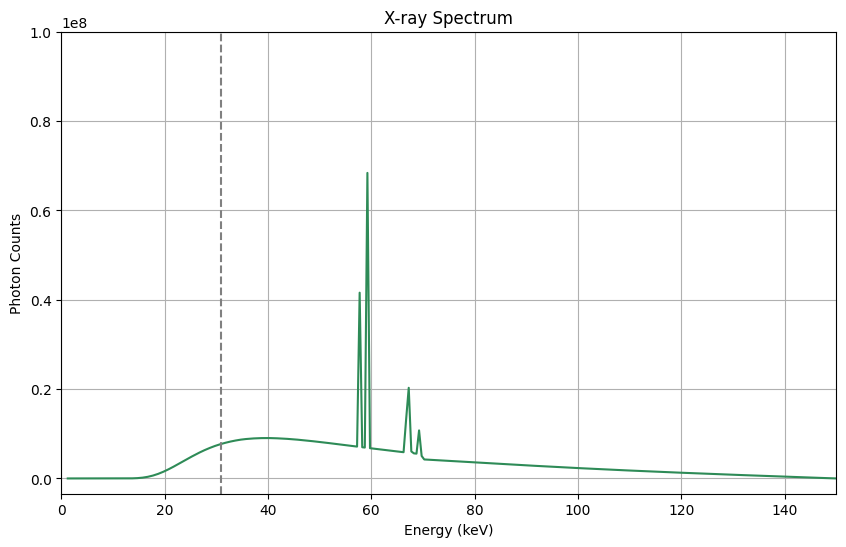
\includegraphics[width=\linewidth]{typicalxrayspectra.png}
	\caption{X-ray Spectrum from a X-ray tube with a Tungsten target}
  \label{fig:basespectra}
\end{figure}

In Figure \ref{fig:basespectra} we can clearly see the sharp characteristic peaks that correspond to Tungsten. Writing code for filtering using NIST data and interpolation to fit the number of data points required., 

\begin{python}
import pandas as pd
from scipy.interpolate import interp1d

# Load csv
bone_data = pd.read_csv("bone.csv", names=["Energy_MeV", "Mu_Rho"], header=None)#

# Convert energy to KeV
bone_data["Energy_KeV"] = bone_data["Energy_MeV"] * 1000

# Average out duplicates by grouping
bone_data = bone_data.groupby("Energy_KeV", as_index=False).mean()

# Convert to linear attenuation (mu = mu/rho * rho)
bone_density = 1.85  # g/cm^3
bone_data["Mu"] = bone_data["Mu_Rho"] * bone_density  # [cm^-1]
mu = bone_data["Mu"].to_numpy()

# Create interpolation function for attenuation coefficients
mu_interp = interp1d(bone_data["Energy_KeV"], bone_data["Mu"], bounds_error=False, fill_value="extrapolate")

mu_at_spectrum_energies = mu_interp(energies)

thickness_cm = 0.5
I0 = s.get_spk()

I_filtered = I0 * np.exp(-mu_at_spectrum_energies * thickness_cm)
\end{python}

\begin{figure}[H]
	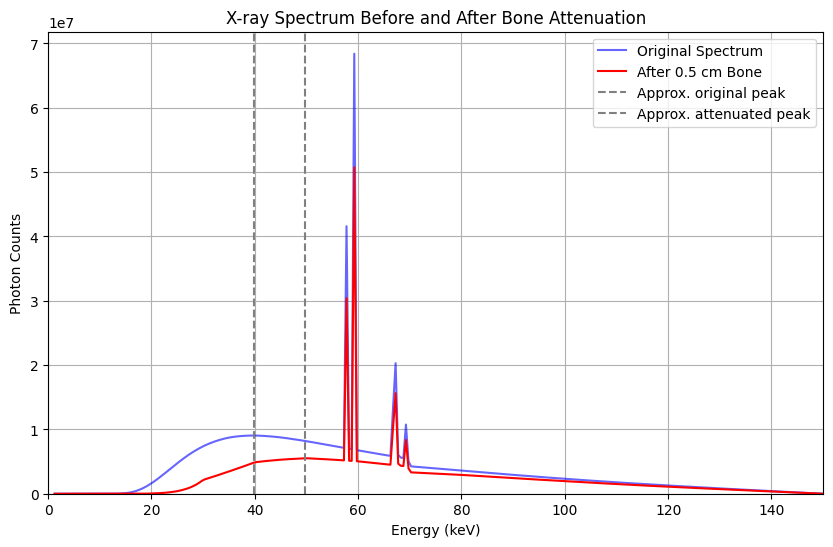
\includegraphics[width=\linewidth]{beamhardening.png}
	\caption{Comparing X-ray spectra before and after passing through 0.5cm of bone}
  \label{fig:beamhardening}
\end{figure}

Figure \ref{fig:beamhardening} clearly shows beam hardening on the X-ray spectrum. The lower-energy (soft) X-rays are preferentially attenuated, resulting in a spectrum that is skewed toward higher energies. Lower-energy photons are absorbed more readily than high-energy ones. As a result, the transmitted spectrum becomes "hardened," with its average energy increasing. We also don't see any hardening for the monochromatic peaks, as expected. 

Beam hardening is significant in image reconstruction, as it may result in characteristic artefacts. CT beam hardening artefacts are known as: streaking artefacts, where dark bands appear between dense structures, and cupping artefacts, where the center of a homogeneous object appears less attenuating than the periphery \cite{Murphy_2016}.

\subsection{Phantoms and Sinograms}
In medical scans, phantoms are used as stand-ins for human tissues to ensure that systems and methods are working correctly. One common such phantom is the Shepp-Logan phantom \cite{Shepp_Logan_1974}. 

\begin{figure}.
	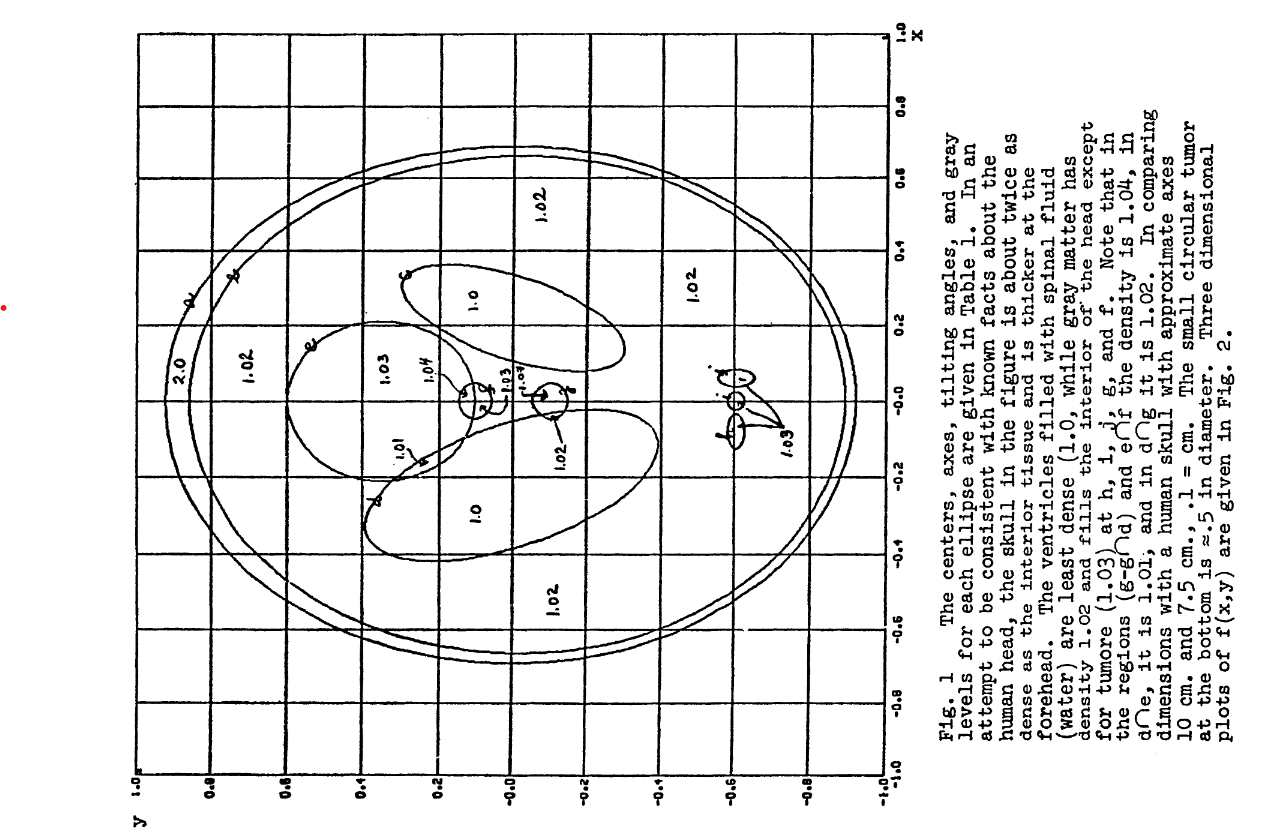
\includegraphics[width=\linewidth]{shepplogan.png}
	\caption{Shepp-Logan head phantom image}
	\label{fig:shepplogan}
\end{figure}

Using Jan Hrach's python code, \cite{phantom_py}, I can recreate the Shepp-Logan phantom with constant attenuation coefficients.

Another phantom I created was a simple circle of bone surrounded by a larger circle of soft tissue. This was an easy way to test using the energy dependent attenuation coefficients.

\begin{python}
def circlemask(radii, centre_x, centre_y, width, height):
    x, y = np.ogrid[:width, :height]
    mask = (x-centre_x)**2 + (y-centre_y)**2 <= radii**2
    return mask
   
width, height = 180,180
s = sp.Spek(kvp=150,th=12)
energies = s.get_k()
# Load each material
mu_bone = load_mu_data(r"code\bone.csv", density=1.85, energy_range_KeV=energies)
mu_tissue = load_mu_data(r"code\soft_tissue.csv", density=1.06, energy_range_KeV=energies)
E=len(energies)

phantom = np.zeros((height, width, E))
bone_mask = circlemask(10,width//2,height//2,width,height)
thigh_mask=circlemask(40,width//2,height//2,width,height)

# Background
phantom[:, :, :] = 0  # broadcast over all pixels

# Thigh region
phantom[thigh_mask, :] = mu_tissue

# Bone region
phantom[bone_mask, :] = mu_bone
\end{python}

We can use matplotlib to display these phantoms:

\begin{figure}[H]
	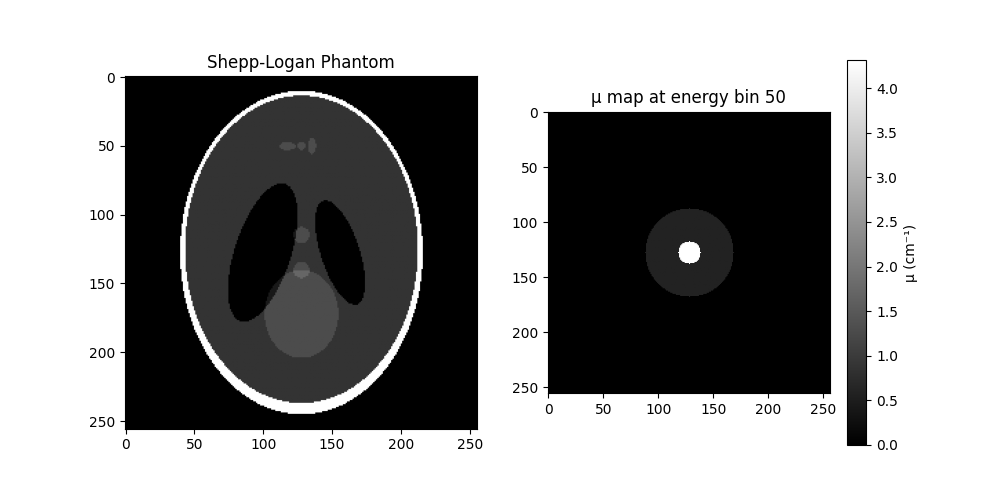
\includegraphics[width=\linewidth]{simplephantom.png}
	\caption{Left: Shepp-Logan phantom. Right: Circular phantom with central bone inclusion ($\mu$ map at energy bin 50).}
	\label{fig:phantoms}
\end{figure}

\bibliography{References}
\bibliographystyle{ieeetr}
\end{document}
